% Options for packages loaded elsewhere
\PassOptionsToPackage{unicode}{hyperref}
\PassOptionsToPackage{hyphens}{url}
\PassOptionsToPackage{dvipsnames,svgnames,x11names}{xcolor}
%
\documentclass[
  letterpaper,
  DIV=11]{scrartcl}

\usepackage{amsmath,amssymb}
\usepackage{iftex}
\ifPDFTeX
  \usepackage[T1]{fontenc}
  \usepackage[utf8]{inputenc}
  \usepackage{textcomp} % provide euro and other symbols
\else % if luatex or xetex
  \usepackage{unicode-math}
  \defaultfontfeatures{Scale=MatchLowercase}
  \defaultfontfeatures[\rmfamily]{Ligatures=TeX,Scale=1}
\fi
\usepackage{lmodern}
\ifPDFTeX\else  
    % xetex/luatex font selection
\fi
% Use upquote if available, for straight quotes in verbatim environments
\IfFileExists{upquote.sty}{\usepackage{upquote}}{}
\IfFileExists{microtype.sty}{% use microtype if available
  \usepackage[]{microtype}
  \UseMicrotypeSet[protrusion]{basicmath} % disable protrusion for tt fonts
}{}
\makeatletter
\@ifundefined{KOMAClassName}{% if non-KOMA class
  \IfFileExists{parskip.sty}{%
    \usepackage{parskip}
  }{% else
    \setlength{\parindent}{0pt}
    \setlength{\parskip}{6pt plus 2pt minus 1pt}}
}{% if KOMA class
  \KOMAoptions{parskip=half}}
\makeatother
\usepackage{xcolor}
\setlength{\emergencystretch}{3em} % prevent overfull lines
\setcounter{secnumdepth}{5}
% Make \paragraph and \subparagraph free-standing
\ifx\paragraph\undefined\else
  \let\oldparagraph\paragraph
  \renewcommand{\paragraph}[1]{\oldparagraph{#1}\mbox{}}
\fi
\ifx\subparagraph\undefined\else
  \let\oldsubparagraph\subparagraph
  \renewcommand{\subparagraph}[1]{\oldsubparagraph{#1}\mbox{}}
\fi

\usepackage{color}
\usepackage{fancyvrb}
\newcommand{\VerbBar}{|}
\newcommand{\VERB}{\Verb[commandchars=\\\{\}]}
\DefineVerbatimEnvironment{Highlighting}{Verbatim}{commandchars=\\\{\}}
% Add ',fontsize=\small' for more characters per line
\usepackage{framed}
\definecolor{shadecolor}{RGB}{241,243,245}
\newenvironment{Shaded}{\begin{snugshade}}{\end{snugshade}}
\newcommand{\AlertTok}[1]{\textcolor[rgb]{0.68,0.00,0.00}{#1}}
\newcommand{\AnnotationTok}[1]{\textcolor[rgb]{0.37,0.37,0.37}{#1}}
\newcommand{\AttributeTok}[1]{\textcolor[rgb]{0.40,0.45,0.13}{#1}}
\newcommand{\BaseNTok}[1]{\textcolor[rgb]{0.68,0.00,0.00}{#1}}
\newcommand{\BuiltInTok}[1]{\textcolor[rgb]{0.00,0.23,0.31}{#1}}
\newcommand{\CharTok}[1]{\textcolor[rgb]{0.13,0.47,0.30}{#1}}
\newcommand{\CommentTok}[1]{\textcolor[rgb]{0.37,0.37,0.37}{#1}}
\newcommand{\CommentVarTok}[1]{\textcolor[rgb]{0.37,0.37,0.37}{\textit{#1}}}
\newcommand{\ConstantTok}[1]{\textcolor[rgb]{0.56,0.35,0.01}{#1}}
\newcommand{\ControlFlowTok}[1]{\textcolor[rgb]{0.00,0.23,0.31}{#1}}
\newcommand{\DataTypeTok}[1]{\textcolor[rgb]{0.68,0.00,0.00}{#1}}
\newcommand{\DecValTok}[1]{\textcolor[rgb]{0.68,0.00,0.00}{#1}}
\newcommand{\DocumentationTok}[1]{\textcolor[rgb]{0.37,0.37,0.37}{\textit{#1}}}
\newcommand{\ErrorTok}[1]{\textcolor[rgb]{0.68,0.00,0.00}{#1}}
\newcommand{\ExtensionTok}[1]{\textcolor[rgb]{0.00,0.23,0.31}{#1}}
\newcommand{\FloatTok}[1]{\textcolor[rgb]{0.68,0.00,0.00}{#1}}
\newcommand{\FunctionTok}[1]{\textcolor[rgb]{0.28,0.35,0.67}{#1}}
\newcommand{\ImportTok}[1]{\textcolor[rgb]{0.00,0.46,0.62}{#1}}
\newcommand{\InformationTok}[1]{\textcolor[rgb]{0.37,0.37,0.37}{#1}}
\newcommand{\KeywordTok}[1]{\textcolor[rgb]{0.00,0.23,0.31}{#1}}
\newcommand{\NormalTok}[1]{\textcolor[rgb]{0.00,0.23,0.31}{#1}}
\newcommand{\OperatorTok}[1]{\textcolor[rgb]{0.37,0.37,0.37}{#1}}
\newcommand{\OtherTok}[1]{\textcolor[rgb]{0.00,0.23,0.31}{#1}}
\newcommand{\PreprocessorTok}[1]{\textcolor[rgb]{0.68,0.00,0.00}{#1}}
\newcommand{\RegionMarkerTok}[1]{\textcolor[rgb]{0.00,0.23,0.31}{#1}}
\newcommand{\SpecialCharTok}[1]{\textcolor[rgb]{0.37,0.37,0.37}{#1}}
\newcommand{\SpecialStringTok}[1]{\textcolor[rgb]{0.13,0.47,0.30}{#1}}
\newcommand{\StringTok}[1]{\textcolor[rgb]{0.13,0.47,0.30}{#1}}
\newcommand{\VariableTok}[1]{\textcolor[rgb]{0.07,0.07,0.07}{#1}}
\newcommand{\VerbatimStringTok}[1]{\textcolor[rgb]{0.13,0.47,0.30}{#1}}
\newcommand{\WarningTok}[1]{\textcolor[rgb]{0.37,0.37,0.37}{\textit{#1}}}

\providecommand{\tightlist}{%
  \setlength{\itemsep}{0pt}\setlength{\parskip}{0pt}}\usepackage{longtable,booktabs,array}
\usepackage{calc} % for calculating minipage widths
% Correct order of tables after \paragraph or \subparagraph
\usepackage{etoolbox}
\makeatletter
\patchcmd\longtable{\par}{\if@noskipsec\mbox{}\fi\par}{}{}
\makeatother
% Allow footnotes in longtable head/foot
\IfFileExists{footnotehyper.sty}{\usepackage{footnotehyper}}{\usepackage{footnote}}
\makesavenoteenv{longtable}
\usepackage{graphicx}
\makeatletter
\def\maxwidth{\ifdim\Gin@nat@width>\linewidth\linewidth\else\Gin@nat@width\fi}
\def\maxheight{\ifdim\Gin@nat@height>\textheight\textheight\else\Gin@nat@height\fi}
\makeatother
% Scale images if necessary, so that they will not overflow the page
% margins by default, and it is still possible to overwrite the defaults
% using explicit options in \includegraphics[width, height, ...]{}
\setkeys{Gin}{width=\maxwidth,height=\maxheight,keepaspectratio}
% Set default figure placement to htbp
\makeatletter
\def\fps@figure{htbp}
\makeatother
\newlength{\cslhangindent}
\setlength{\cslhangindent}{1.5em}
\newlength{\csllabelwidth}
\setlength{\csllabelwidth}{3em}
\newlength{\cslentryspacingunit} % times entry-spacing
\setlength{\cslentryspacingunit}{\parskip}
\newenvironment{CSLReferences}[2] % #1 hanging-ident, #2 entry spacing
 {% don't indent paragraphs
  \setlength{\parindent}{0pt}
  % turn on hanging indent if param 1 is 1
  \ifodd #1
  \let\oldpar\par
  \def\par{\hangindent=\cslhangindent\oldpar}
  \fi
  % set entry spacing
  \setlength{\parskip}{#2\cslentryspacingunit}
 }%
 {}
\usepackage{calc}
\newcommand{\CSLBlock}[1]{#1\hfill\break}
\newcommand{\CSLLeftMargin}[1]{\parbox[t]{\csllabelwidth}{#1}}
\newcommand{\CSLRightInline}[1]{\parbox[t]{\linewidth - \csllabelwidth}{#1}\break}
\newcommand{\CSLIndent}[1]{\hspace{\cslhangindent}#1}

\usepackage{booktabs}
\usepackage{longtable}
\usepackage{array}
\usepackage{multirow}
\usepackage{wrapfig}
\usepackage{float}
\usepackage{colortbl}
\usepackage{pdflscape}
\usepackage{tabu}
\usepackage{threeparttable}
\usepackage{threeparttablex}
\usepackage[normalem]{ulem}
\usepackage{makecell}
\usepackage{xcolor}
\KOMAoption{captions}{tableheading}
\makeatletter
\@ifpackageloaded{tcolorbox}{}{\usepackage[skins,breakable]{tcolorbox}}
\@ifpackageloaded{fontawesome5}{}{\usepackage{fontawesome5}}
\definecolor{quarto-callout-color}{HTML}{909090}
\definecolor{quarto-callout-note-color}{HTML}{0758E5}
\definecolor{quarto-callout-important-color}{HTML}{CC1914}
\definecolor{quarto-callout-warning-color}{HTML}{EB9113}
\definecolor{quarto-callout-tip-color}{HTML}{00A047}
\definecolor{quarto-callout-caution-color}{HTML}{FC5300}
\definecolor{quarto-callout-color-frame}{HTML}{acacac}
\definecolor{quarto-callout-note-color-frame}{HTML}{4582ec}
\definecolor{quarto-callout-important-color-frame}{HTML}{d9534f}
\definecolor{quarto-callout-warning-color-frame}{HTML}{f0ad4e}
\definecolor{quarto-callout-tip-color-frame}{HTML}{02b875}
\definecolor{quarto-callout-caution-color-frame}{HTML}{fd7e14}
\makeatother
\makeatletter
\makeatother
\makeatletter
\makeatother
\makeatletter
\@ifpackageloaded{caption}{}{\usepackage{caption}}
\AtBeginDocument{%
\ifdefined\contentsname
  \renewcommand*\contentsname{Inhaltsverzeichnis}
\else
  \newcommand\contentsname{Inhaltsverzeichnis}
\fi
\ifdefined\listfigurename
  \renewcommand*\listfigurename{Abbildungsverzeichnis}
\else
  \newcommand\listfigurename{Abbildungsverzeichnis}
\fi
\ifdefined\listtablename
  \renewcommand*\listtablename{Tabellenverzeichnis}
\else
  \newcommand\listtablename{Tabellenverzeichnis}
\fi
\ifdefined\figurename
  \renewcommand*\figurename{Abbildung}
\else
  \newcommand\figurename{Abbildung}
\fi
\ifdefined\tablename
  \renewcommand*\tablename{Tabelle}
\else
  \newcommand\tablename{Tabelle}
\fi
}
\@ifpackageloaded{float}{}{\usepackage{float}}
\floatstyle{ruled}
\@ifundefined{c@chapter}{\newfloat{codelisting}{h}{lop}}{\newfloat{codelisting}{h}{lop}[chapter]}
\floatname{codelisting}{Listing}
\newcommand*\listoflistings{\listof{codelisting}{Listingverzeichnis}}
\usepackage{amsthm}
\theoremstyle{definition}
\newtheorem{example}{Beispiel}[section]
\theoremstyle{remark}
\AtBeginDocument{\renewcommand*{\proofname}{Beweis}}
\newtheorem*{remark}{Anmerkung}
\newtheorem*{solution}{Lösung}
\makeatother
\makeatletter
\@ifpackageloaded{caption}{}{\usepackage{caption}}
\@ifpackageloaded{subcaption}{}{\usepackage{subcaption}}
\makeatother
\makeatletter
\@ifpackageloaded{tcolorbox}{}{\usepackage[skins,breakable]{tcolorbox}}
\makeatother
\makeatletter
\@ifundefined{shadecolor}{\definecolor{shadecolor}{rgb}{.97, .97, .97}}
\makeatother
\makeatletter
\makeatother
\makeatletter
\makeatother
\ifLuaTeX
\usepackage[bidi=basic]{babel}
\else
\usepackage[bidi=default]{babel}
\fi
\babelprovide[main,import]{ngerman}
% get rid of language-specific shorthands (see #6817):
\let\LanguageShortHands\languageshorthands
\def\languageshorthands#1{}
\ifLuaTeX
  \usepackage{selnolig}  % disable illegal ligatures
\fi
\IfFileExists{bookmark.sty}{\usepackage{bookmark}}{\usepackage{hyperref}}
\IfFileExists{xurl.sty}{\usepackage{xurl}}{} % add URL line breaks if available
\urlstyle{same} % disable monospaced font for URLs
\hypersetup{
  pdftitle={Einführung in R und RStudio},
  pdfauthor={Daniela Palleschi},
  pdflang={de},
  colorlinks=true,
  linkcolor={blue},
  filecolor={Maroon},
  citecolor={Blue},
  urlcolor={Blue},
  pdfcreator={LaTeX via pandoc}}

\title{Einführung in R und RStudio}
\author{Daniela Palleschi}
\date{Vorlesung Mi. den 18.10.2023}

\begin{document}
\maketitle
\ifdefined\Shaded\renewenvironment{Shaded}{\begin{tcolorbox}[interior hidden, breakable, boxrule=0pt, borderline west={3pt}{0pt}{shadecolor}, enhanced, frame hidden, sharp corners]}{\end{tcolorbox}}\fi

\renewcommand*\contentsname{Inhaltsverzeichnis}
{
\hypersetup{linkcolor=}
\setcounter{tocdepth}{3}
\tableofcontents
}
\hypertarget{wiederholung}{%
\section*{Wiederholung}\label{wiederholung}}

Last week we\ldots{}

\begin{itemize}
\tightlist
\item
  installed R and RStudio
\item
  created our first R script
\item
  did simple arithmetic with objects and vectors
\end{itemize}

\hypertarget{wiederholung-1}{%
\subsection*{Wiederholung}\label{wiederholung-1}}

\begin{Shaded}
\begin{Highlighting}[]
\NormalTok{x }\OtherTok{\textless{}{-}} \FunctionTok{c}\NormalTok{(}\DecValTok{1}\NormalTok{,}\DecValTok{2}\NormalTok{,}\DecValTok{3}\NormalTok{)}
\NormalTok{y }\OtherTok{\textless{}{-}} \FunctionTok{sum}\NormalTok{(}\DecValTok{1}\NormalTok{,}\DecValTok{2}\NormalTok{,}\DecValTok{3}\NormalTok{)}
\end{Highlighting}
\end{Shaded}

\begin{itemize}
\item
  what do the vectors \texttt{x} and \texttt{y} contain?
\item
  The object \texttt{x} contains \texttt{1,\ 2,\ 3}.
\item
  The object \texttt{y} contains \texttt{6}.
\end{itemize}

\hypertarget{heutige-ziele}{%
\section*{Heutige Ziele}\label{heutige-ziele}}
\addcontentsline{toc}{section}{Heutige Ziele}

Today we will learn\ldots{}

\begin{itemize}
\tightlist
\item
  what dataframes are
\item
  the difference between categorical and continuous data
\item
  how to produce plots with \texttt{ggplot}
\item
  choose the right plot for our data
\end{itemize}

\hypertarget{lust-auf-mehr}{%
\subsection*{Lust auf mehr?}\label{lust-auf-mehr}}
\addcontentsline{toc}{subsection}{Lust auf mehr?}

\begin{itemize}
\tightlist
\item
  Chapter 2 (Data Visualisation) in Wickham et al. (2023), up until
  section 2.4
\item
  Chapter 3 (Data Visualisation) in Nordmann \& DeBruine (2022)
\end{itemize}

\hypertarget{vorbereitung}{%
\subsection*{Vorbereitung}\label{vorbereitung}}
\addcontentsline{toc}{subsection}{Vorbereitung}

In your RProject folder\ldots{}

\begin{itemize}
\tightlist
\item
  create a new folder called \texttt{moodle}

  \begin{itemize}
  \tightlist
  \item
    download the Moodle materials from today and save them there
  \end{itemize}
\item
  create a new folder in \texttt{notes} called \texttt{02-datenviz1}
\item
  open a new \texttt{.R} script

  \begin{itemize}
  \tightlist
  \item
    save it in the new folder
  \end{itemize}
\end{itemize}

\hypertarget{packages}{%
\subsubsection{Packages}\label{packages}}

\begin{itemize}
\tightlist
\item
  Pakete (installiert und) ladt

  \begin{itemize}
  \tightlist
  \item
    \texttt{tidyverse}
  \item
    \texttt{languageR}
  \item
    \texttt{ggthemes}
  \item
    \texttt{patchwork}
  \end{itemize}
\end{itemize}

\begin{Shaded}
\begin{Highlighting}[]
\CommentTok{\# in the CONSOLE: install packages if needed}
\FunctionTok{install.packages}\NormalTok{(}\StringTok{"tidyverse"}\NormalTok{)}
\FunctionTok{install.packages}\NormalTok{(}\StringTok{"languageR"}\NormalTok{)}
\FunctionTok{install.packages}\NormalTok{(}\StringTok{"ggthemes"}\NormalTok{) }\CommentTok{\# for customising our plots}
\FunctionTok{install.packages}\NormalTok{(}\StringTok{"patchwork"}\NormalTok{) }\CommentTok{\# plot layouts}
\end{Highlighting}
\end{Shaded}

\begin{Shaded}
\begin{Highlighting}[]
\CommentTok{\# Pakete laden}
\FunctionTok{library}\NormalTok{(tidyverse)}
\FunctionTok{library}\NormalTok{(languageR)}
\FunctionTok{library}\NormalTok{(ggthemes)}
\FunctionTok{library}\NormalTok{(patchwork)}
\end{Highlighting}
\end{Shaded}

\hypertarget{data-frames}{%
\section{Data frames}\label{data-frames}}

\begin{itemize}
\item
  data frames are a collection of variables, where

  \begin{itemize}
  \tightlist
  \item
    each variable is one column
  \item
    each row is a single observation/data point
  \item
    each cell in a row is linked
  \end{itemize}
\item
  data frames are just like spreadsheets, but are rectangular
\item
  different words for data frames:

  \begin{itemize}
  \tightlist
  \item
    data frame
  \item
    dataset
  \item
    tibble (in the \texttt{tidyverse})
  \end{itemize}
\end{itemize}

\hypertarget{talking-about-datasets}{%
\subsection{Talking about datasets}\label{talking-about-datasets}}

\begin{itemize}
\item
  when we talk about our data, we use certan words to refer to different
  parts:
\item
  a \textbf{variable}: a quantity, quality, or property you can measure
\item
  a \textbf{value}: the state of a variable when you measure it
\item
  an \textbf{observation}: set of measurements made under similar
  conditions

  \begin{itemize}
  \tightlist
  \item
    will contain several values each associated with a variable
  \item
    an observation for a single variable is sometimes called a
    \emph{data point}
  \end{itemize}
\item
  \textbf{tabular data} is a set of values, each associated with a
  variable and an observation

  \begin{itemize}
  \tightlist
  \item
    tabular data is \emph{tidy} if each value is placed in its own
    \emph{cell}, each variable in its own column, and each observation
    in its own row
  \end{itemize}
\end{itemize}

\hypertarget{categorical-and-continuous-variables}{%
\subsection{Categorical and continuous
variables}\label{categorical-and-continuous-variables}}

\begin{itemize}
\tightlist
\item
  how we visual the distribution of a variable depends on what type of
  data it represents: \emph{categorical} or \emph{numerical}
\item
  a variable is \emph{categorical} if it can take a small set of values
  that can be grouped together
\item
  e.g., old/young, short/tall, grammatical/ungrammatical, L1/L2-speaker
\item
  a variable is \emph{numerical} (i.e., quantitative) if it can take on
  a wide range of numerical values

  \begin{itemize}
  \tightlist
  \item
    and it would make sense to add, subtract, compute the mean, etc.
  \item
    can be \emph{continuous} (decimal points make sense, e.g., 1.5cm)
  \item
    or \emph{discrete} (decimal points do \emph{not} make sense, e.g.,
    1.5 children doesn't make sense)
  \item
    age, height, reaction times, format frequencies
  \end{itemize}
\item
  we produce different plots depending on what type of variables we want
  to visualise
\end{itemize}

\hypertarget{lexical-decision-task}{%
\section{Lexical Decision Task}\label{lexical-decision-task}}

\begin{itemize}
\item
  our first dataset contains data from a lexical decision task (LDT)
\item
  in the LDT, participants press a button to indicate whether a word is
  a real word or a pseudoword
\end{itemize}

\begin{figure}

{\centering 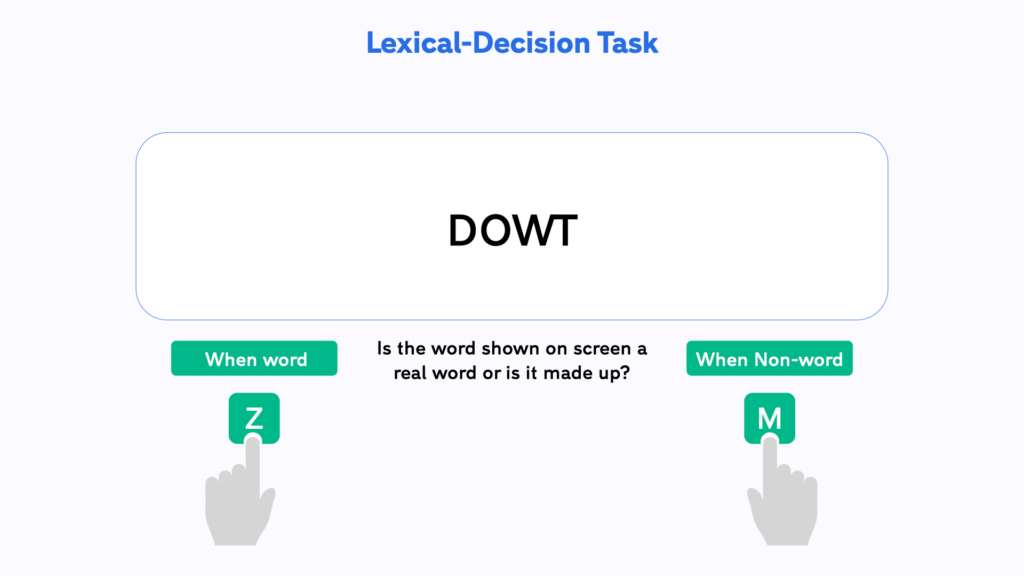
\includegraphics[width=1\textwidth,height=\textheight]{_intro_r_slides_files/figure-pdf/unnamed-chunk-7-1.png}

}

\caption{Source:
https://www.testable.org/wp-content/uploads/2022/11/Lexical\_decision\_task-1024x576.png}

\end{figure}

\begin{figure}

{\centering 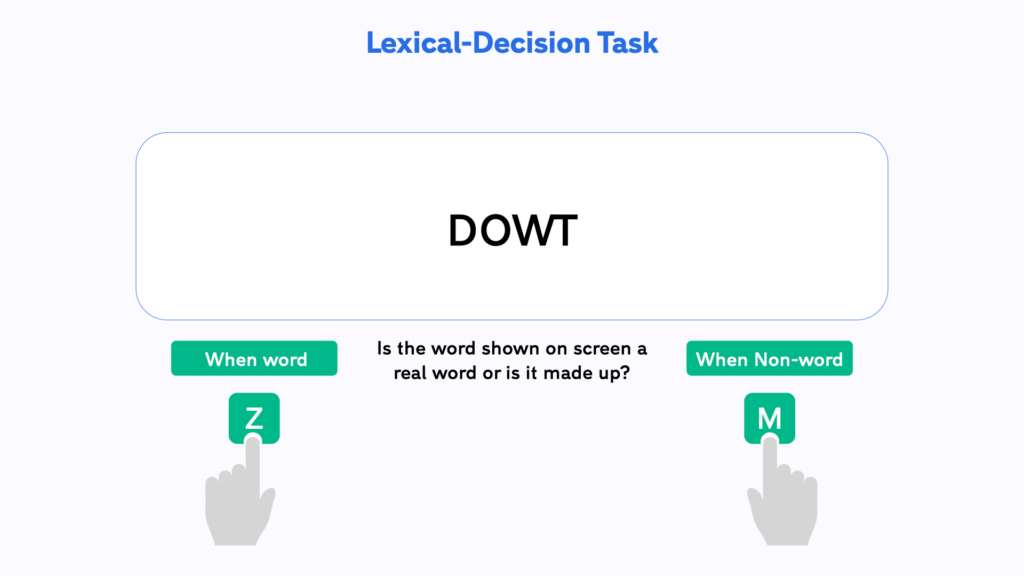
\includegraphics[width=1\textwidth,height=\textheight]{_intro_r_slides_files/figure-pdf/unnamed-chunk-8-1.png}

}

\end{figure}

\hypertarget{ldt-variables}{%
\subsection{LDT variables}\label{ldt-variables}}

\begin{itemize}
\tightlist
\item
  common variables collected in a lexical decision task experiment are:

  \begin{itemize}
  \tightlist
  \item
    reaction time
  \item
    accuracy (correct/incorrect)
  \item
    word category (e.g., real/pseudo, noun/verb)
  \item
    word frequency
  \end{itemize}
\item
  additional variables that might be collected could be:

  \begin{itemize}
  \tightlist
  \item
    participant demographics (e.g., age, L1/L2, gender)
  \end{itemize}
\end{itemize}

\hypertarget{lexdec-dataset}{%
\section{\texorpdfstring{\texttt{lexdec}
dataset}{lexdec dataset}}\label{lexdec-dataset}}

\begin{itemize}
\tightlist
\item
  \texttt{languageR} is a companion package for the textbook
  (\textbf{baayen\_analyzing\_2008?})

  \begin{itemize}
  \tightlist
  \item
    contains linguistic datasets, e.g., \texttt{lexdec}
  \end{itemize}
\item
  the \texttt{lexdec} dataset contains data for a lexical decision task
  in English

  \begin{itemize}
  \tightlist
  \item
    we will be working with variables such as reaction times and
    accuracy
  \end{itemize}
\end{itemize}

\hypertarget{lexdec-variables}{%
\subsection{\texorpdfstring{\texttt{lexdec}
variables}{lexdec variables}}\label{lexdec-variables}}

\begin{itemize}
\tightlist
\item
  a list of some of the variables is included in
  Tabelle~\ref{tbl-lexdec}
\end{itemize}

\hypertarget{tbl-lexdec}{}
\begin{table}
\caption{\label{tbl-lexdec}Data dictionary for \texttt{df\_lexdec}: Lexical decision latencies
elicited from 21 subjects for 79 English concrete nouns, with variables
linked to subject or word. }\tabularnewline

\centering
\begin{tabular}{l|l}
\hline
variable & description\\
\hline
Subject & a factor for the subjects\\
\hline
RT & a numeric vector for reaction times in milliseconds\\
\hline
Trial & a numeric vector for the rank of the trial in the experimental list.\\
\hline
Sex & a factor with levels F (female) and M (male).\\
\hline
NativeLanguage & a factor with levels English and Other, distinguishing between native and nonnative speakers of English\\
\hline
\end{tabular}
\end{table}

\hypertarget{ldt-research-questions}{%
\subsection{LDT research questions}\label{ldt-research-questions}}

\begin{itemize}
\tightlist
\item
  before we conduct an experiment, we have research questions that we
  want to answer with the data

  \begin{itemize}
  \tightlist
  \item
    today we'll address the following question:

    \begin{itemize}
    \tightlist
    \item
      do the reaction times differ between native and non-native
      speakers?
    \end{itemize}
  \end{itemize}
\end{itemize}

\hypertarget{load-the-data}{%
\subsection{Load the data}\label{load-the-data}}

\begin{itemize}
\tightlist
\item
  our data is available in the \texttt{lanaugeR} package we've already
  loaded

  \begin{itemize}
  \tightlist
  \item
    to print the data, just type the name of the dataset and run it
  \end{itemize}
\item
  below we only see a few variables, but you should see more in your
  console
\end{itemize}

\begin{Shaded}
\begin{Highlighting}[]
\NormalTok{lexdec}
\end{Highlighting}
\end{Shaded}

\begin{verbatim}
  Subject       RT Trial Sex NativeLanguage Correct PrevType PrevCorrect
1      A1 6.340359    23   F        English correct     word     correct
2      A1 6.308098    27   F        English correct  nonword     correct
3      A1 6.349139    29   F        English correct  nonword     correct
4      A1 6.186209    30   F        English correct     word     correct
5      A1 6.025866    32   F        English correct  nonword     correct
6      A1 6.180017    33   F        English correct     word     correct
\end{verbatim}

\begin{itemize}
\tightlist
\item
  how many variables do we have? observations?
\end{itemize}

\hypertarget{save-data-as-an-object}{%
\subsubsection{Save data as an object}\label{save-data-as-an-object}}

\begin{itemize}
\tightlist
\item
  to save the data in our Environment, we have to assign it a name

  \begin{itemize}
  \tightlist
  \item
    let's call it \texttt{df\_lexdec}, which means ``data frame lexical
    decision''
  \end{itemize}
\end{itemize}

\begin{Shaded}
\begin{Highlighting}[]
\NormalTok{df\_lexdec }\OtherTok{\textless{}{-}}\NormalTok{ lexdec}
\end{Highlighting}
\end{Shaded}

\begin{itemize}
\tightlist
\item
  now we see it in our Enrivonment

  \begin{itemize}
  \tightlist
  \item
    double-click on it to view it in the Editor pane
  \end{itemize}
\end{itemize}

\hypertarget{relevant-variables}{%
\subsection{Relevant variables}\label{relevant-variables}}

\begin{itemize}
\tightlist
\item
  Among the variables we have are:

  \begin{enumerate}
  \def\labelenumi{\arabic{enumi}.}
  \tightlist
  \item
    \textbf{Subject}: participant ID
  \item
    \textbf{RT}: logged reaction times
  \item
    \textbf{NativeLanguage}: the native language of the participant
  \item
    \textbf{Word}: what word was presented
  \item
    \textbf{Class}: if the word was animal or plant
  \end{enumerate}
\end{itemize}

\begin{tcolorbox}[enhanced jigsaw, colbacktitle=quarto-callout-tip-color!10!white, rightrule=.15mm, toptitle=1mm, bottomtitle=1mm, breakable, leftrule=.75mm, toprule=.15mm, left=2mm, coltitle=black, opacitybacktitle=0.6, title=\textcolor{quarto-callout-tip-color}{\faLightbulb}\hspace{0.5em}{Aufgabe~\ref{exm-help}: \texttt{?lexdec}}, colback=white, titlerule=0mm, arc=.35mm, bottomrule=.15mm, opacityback=0, colframe=quarto-callout-tip-color-frame]

\begin{example}[]\protect\hypertarget{exm-help}{}\label{exm-help}

~

Find out what the other variables represent by running \texttt{?lexdec}
in the console.

\end{example}

\end{tcolorbox}

\hypertarget{ultimate-goal}{%
\subsection{Ultimate goal}\label{ultimate-goal}}

\begin{itemize}
\tightlist
\item
  our ultimate goal today is to produce the following visualisation of
  the data

  \begin{itemize}
  \tightlist
  \item
    the plot shows the distribution (\texttt{count}) of reaction times
    and native language of the participants
  \end{itemize}
\end{itemize}

\begin{figure}[centre]

{\centering 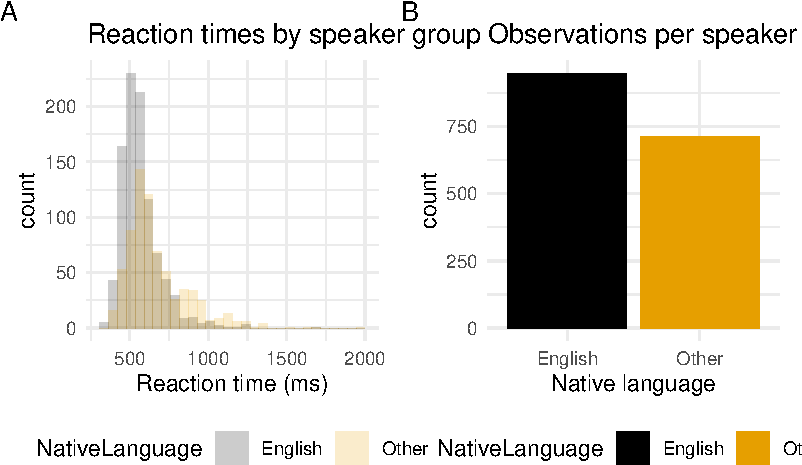
\includegraphics{_intro_r_slides_files/figure-pdf/unnamed-chunk-13-1.pdf}

}

\end{figure}

\hypertarget{creating-plots-with-ggplot2}{%
\section{\texorpdfstring{Creating plots with
\texttt{ggplot2}}{Creating plots with ggplot2}}\label{creating-plots-with-ggplot2}}

\begin{itemize}
\tightlist
\item
  the \texttt{tidyverse} is a collection of packages that facilitate
  data tidying and visualisation

  \begin{itemize}
  \tightlist
  \item
    when we load the \texttt{tidyverse}, this collection of packages is
    automatically loaded
  \end{itemize}
\item
  the \texttt{ggplot2} package is a \texttt{tidyverse} package that
  builds plots in layers
\end{itemize}

\begin{figure}

{\centering \includegraphics[width=0.7\textwidth,height=\textheight]{../../media/Nordmann_3dataviz_layers.png}

}

\caption{\href{https://psyteachr.github.io/ads-v2/03-viz.html}{Image
source:} Nordmann \& DeBruine (2022) (all rights reserved)}

\end{figure}

\hypertarget{layer-1-empty-canvas}{%
\subsection{Layer 1: empty canvas}\label{layer-1-empty-canvas}}

\begin{itemize}
\tightlist
\item
  the first layer with the function \texttt{ggplot()} is like an empty
  canvas
\end{itemize}

\begin{Shaded}
\begin{Highlighting}[]
\FunctionTok{ggplot}\NormalTok{(}\AttributeTok{data =}\NormalTok{ df\_lexdec)}
\end{Highlighting}
\end{Shaded}

\begin{figure}[H]

{\centering 
\includegraphics{_intro_r_slides_files/figure-pdf/unnamed-chunk-16-1.pdf}

}

\end{figure}

\hypertarget{layer-2-mapping-aesthetics}{%
\subsection{Layer 2: mapping
aesthetics}\label{layer-2-mapping-aesthetics}}

\begin{itemize}
\tightlist
\item
  next we tell \texttt{ggplot()} how to visually represent our variables

  \begin{itemize}
  \tightlist
  \item
    we use the \texttt{mapping} argument of \texttt{ggplot()} to define
    how variables are \emph{mapped} to visual properties
    (\emph{aesthetics})
  \end{itemize}
\item
  for our first plot, we want to map reaction times (\texttt{RT}) on the
  x-axis (the bottom of the plot)

  \begin{itemize}
  \tightlist
  \item
    we wrap the logged \texttt{RT} in the \texttt{exp()} function to get
    RTs in milliseconds (for reasons we won't discuss)
  \end{itemize}
\end{itemize}

\begin{Shaded}
\begin{Highlighting}[]
\FunctionTok{ggplot}\NormalTok{(}\AttributeTok{data =}\NormalTok{ df\_lexdec) }\SpecialCharTok{+}
  \FunctionTok{aes}\NormalTok{(}\AttributeTok{x =} \FunctionTok{exp}\NormalTok{(RT))}
\end{Highlighting}
\end{Shaded}

\begin{figure}[H]

{\centering 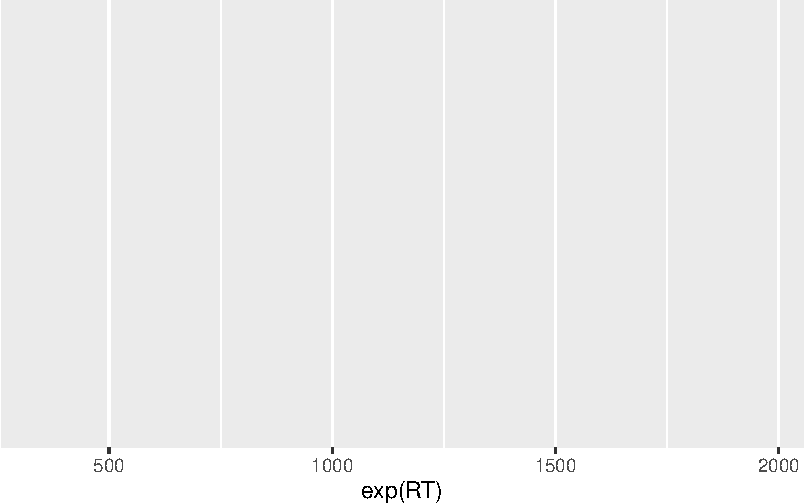
\includegraphics{_intro_r_slides_files/figure-pdf/unnamed-chunk-17-1.pdf}

}

\end{figure}

\begin{tcolorbox}[enhanced jigsaw, colbacktitle=quarto-callout-tip-color!10!white, rightrule=.15mm, toptitle=1mm, bottomtitle=1mm, breakable, leftrule=.75mm, toprule=.15mm, left=2mm, coltitle=black, opacitybacktitle=0.6, title=\textcolor{quarto-callout-tip-color}{\faLightbulb}\hspace{0.5em}{Aufgabe~\ref{exm-layer2}: Mapping aesthetics}, colback=white, titlerule=0mm, arc=.35mm, bottomrule=.15mm, opacityback=0, colframe=quarto-callout-tip-color-frame]

\begin{example}[]\protect\hypertarget{exm-layer2}{}\label{exm-layer2}

~

\begin{enumerate}
\def\labelenumi{\arabic{enumi}.}
\tightlist
\item
  Produce the plot so far
\end{enumerate}

\end{example}

\end{tcolorbox}

\hypertarget{layer-3-adding-observations}{%
\subsection{Layer 3: adding
observations}\label{layer-3-adding-observations}}

\begin{itemize}
\tightlist
\item
  we don't see any observations (i.e., the bars) on the plot, why not?

  \begin{itemize}
  \tightlist
  \item
    we haven't told \texttt{ggplot()} how to visualise them
  \end{itemize}
\item
  we have to define a \textbf{geom}: the \emph{geom}etrical object that
  a plot uses to represent data

  \begin{itemize}
  \tightlist
  \item
    in \texttt{ggplot2}, geom functions start with \texttt{geom\_}
  \item
    we often describe plots in terms of types of geoms they use, e.g.,
    bar charts use bar geoms (\texttt{geom\_bar()}), line charts use
    line geoms (\texttt{geom\_line()}), scatterplots use a point geom
    (\texttt{geom\_point()}), etc.
  \end{itemize}
\end{itemize}

\begin{itemize}
\tightlist
\item
  let's create our histogram using the geom \texttt{geom\_histogram()}
\end{itemize}

\begin{Shaded}
\begin{Highlighting}[]
\FunctionTok{ggplot}\NormalTok{(}\AttributeTok{data =}\NormalTok{ df\_lexdec) }\SpecialCharTok{+}
  \FunctionTok{aes}\NormalTok{(}\AttributeTok{x =} \FunctionTok{exp}\NormalTok{(RT)) }\SpecialCharTok{+}
  \FunctionTok{geom\_histogram}\NormalTok{()}
\end{Highlighting}
\end{Shaded}

\begin{figure}[H]

{\centering 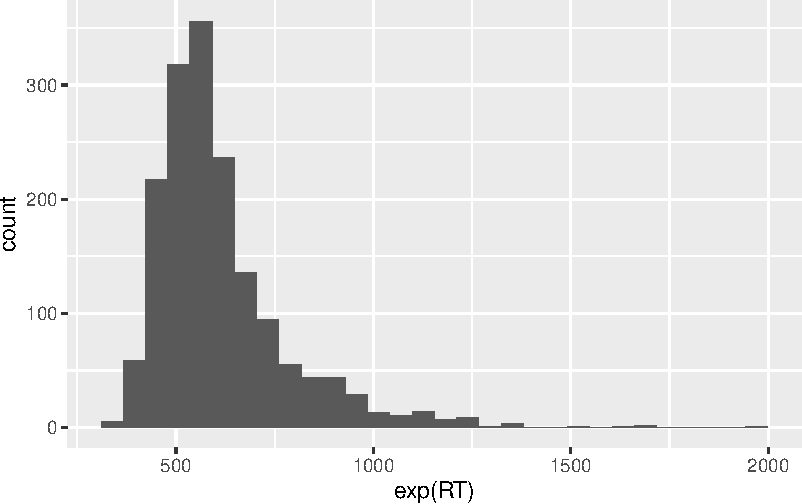
\includegraphics{_intro_r_slides_files/figure-pdf/unnamed-chunk-18-1.pdf}

}

\end{figure}

\begin{tcolorbox}[enhanced jigsaw, colbacktitle=quarto-callout-note-color!10!white, rightrule=.15mm, toptitle=1mm, bottomtitle=1mm, breakable, leftrule=.75mm, toprule=.15mm, left=2mm, coltitle=black, opacitybacktitle=0.6, title=\textcolor{quarto-callout-note-color}{\faInfo}\hspace{0.5em}{Hinweis}, colback=white, titlerule=0mm, arc=.35mm, bottomrule=.15mm, opacityback=0, colframe=quarto-callout-note-color-frame]

We got the following message when including \texttt{geom\_point()}:

\begin{quote}
\texttt{stat\_bin()} using \texttt{bins\ =\ 30}. Pick better value with
\texttt{binwidth}.
\end{quote}

This is just telling us about the width of our bars: each bar represents
a range of possible reaction time values + \texttt{bins\ =\ 30} simply
means there are 30 bars, we can change this have more or fewer bars by
including e.g., \texttt{bins\ =\ 20} or \texttt{bins\ =\ 100} inside
\texttt{geom\_histogram()}

\end{tcolorbox}

\begin{Shaded}
\begin{Highlighting}[]
\FunctionTok{ggplot}\NormalTok{(}
  \AttributeTok{data =}\NormalTok{ df\_lexdec,}
  \AttributeTok{mapping =} \FunctionTok{aes}\NormalTok{(}\AttributeTok{x =} \FunctionTok{exp}\NormalTok{(RT))}
\NormalTok{) }\SpecialCharTok{+}
  \FunctionTok{labs}\NormalTok{(}\AttributeTok{title =} \StringTok{"with geom\_histogram(bins = 20)"}\NormalTok{) }\SpecialCharTok{+}
  \FunctionTok{geom\_histogram}\NormalTok{(}\AttributeTok{bins =} \DecValTok{20}\NormalTok{) }\SpecialCharTok{+}

  \FunctionTok{ggplot}\NormalTok{(}
  \AttributeTok{data =}\NormalTok{ df\_lexdec,}
  \AttributeTok{mapping =} \FunctionTok{aes}\NormalTok{(}\AttributeTok{x =} \FunctionTok{exp}\NormalTok{(RT))}
\NormalTok{) }\SpecialCharTok{+}
  \FunctionTok{labs}\NormalTok{(}\AttributeTok{title =} \StringTok{"with geom\_histogram(bins = 100)"}\NormalTok{) }\SpecialCharTok{+}
  \FunctionTok{geom\_histogram}\NormalTok{(}\AttributeTok{bins =} \DecValTok{100}\NormalTok{)}
\end{Highlighting}
\end{Shaded}

\begin{figure}[H]

{\centering 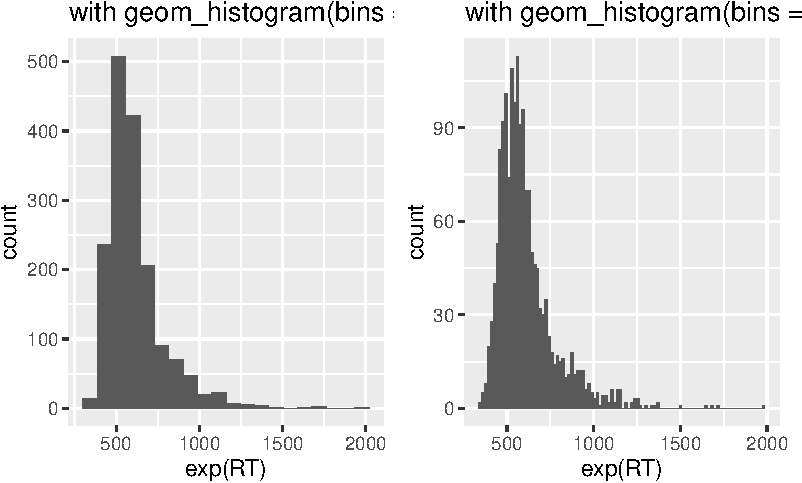
\includegraphics{_intro_r_slides_files/figure-pdf/unnamed-chunk-19-1.pdf}

}

\end{figure}

\hypertarget{adding-aesthetics}{%
\subsection{Adding aesthetics}\label{adding-aesthetics}}

\begin{itemize}
\tightlist
\item
  seeing the distribution of reaction times in general is useful

  \begin{itemize}
  \tightlist
  \item
    but we usually want to compare groups
  \item
    e.g., differences between native and non-native speakers, or between
    types of words
  \end{itemize}
\item
  we also have native language as a variable, how might we visualise
  this in our plot?
\end{itemize}

\begin{Shaded}
\begin{Highlighting}[]
\FunctionTok{ggplot}\NormalTok{(}
  \AttributeTok{data =}\NormalTok{ df\_lexdec,}
  \FunctionTok{aes}\NormalTok{(}\AttributeTok{x =} \FunctionTok{exp}\NormalTok{(RT), }\AttributeTok{fill =}\NormalTok{ NativeLanguage)}
\NormalTok{) }\SpecialCharTok{+}
  \FunctionTok{geom\_histogram}\NormalTok{()}
\end{Highlighting}
\end{Shaded}

\begin{figure}[H]

{\centering 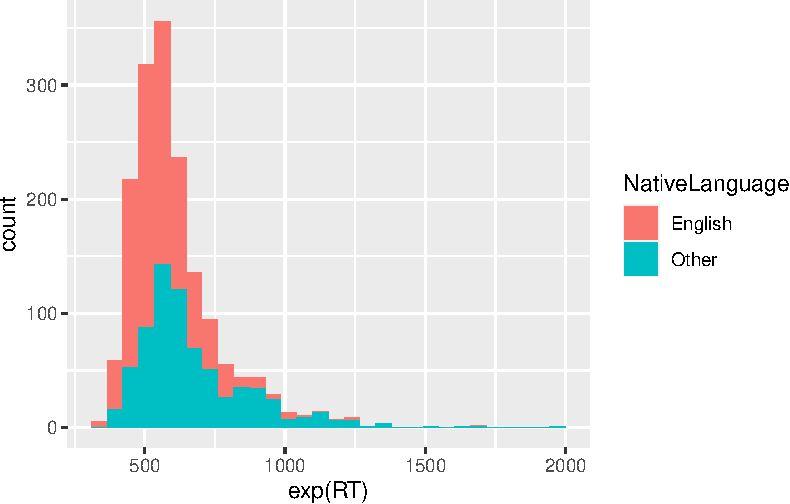
\includegraphics{_intro_r_slides_files/figure-pdf/unnamed-chunk-20-1.pdf}

}

\end{figure}

\begin{itemize}
\tightlist
\item
  we see the red bars and the blue bars, but is the blue histogram
  layered on top of the red?

  \begin{itemize}
  \tightlist
  \item
    or are the red bars stacked in top of the blue bars?
  \end{itemize}
\item
  it's the latter

  \begin{itemize}
  \tightlist
  \item
    let's make is so that the blue histogram is layered on top of the
    red
  \end{itemize}
\end{itemize}

\begin{Shaded}
\begin{Highlighting}[]
\FunctionTok{ggplot}\NormalTok{(}
  \AttributeTok{data =}\NormalTok{ df\_lexdec,}
  \FunctionTok{aes}\NormalTok{(}\AttributeTok{x =} \FunctionTok{exp}\NormalTok{(RT), }\AttributeTok{fill =}\NormalTok{ NativeLanguage)}
\NormalTok{) }\SpecialCharTok{+}
  \FunctionTok{labs}\NormalTok{(}\AttributeTok{title =} \StringTok{"Stacked"}\NormalTok{) }\SpecialCharTok{+}
  \FunctionTok{geom\_histogram}\NormalTok{() }\SpecialCharTok{+} 
  
\FunctionTok{ggplot}\NormalTok{(}
  \AttributeTok{data =}\NormalTok{ df\_lexdec,}
  \FunctionTok{aes}\NormalTok{(}\AttributeTok{x =} \FunctionTok{exp}\NormalTok{(RT), }\AttributeTok{fill =}\NormalTok{ NativeLanguage)}
\NormalTok{) }\SpecialCharTok{+}
  \FunctionTok{labs}\NormalTok{(}\AttributeTok{title =} \StringTok{"Layered: position = }\SpecialCharTok{\textbackslash{}"}\StringTok{identity}\SpecialCharTok{\textbackslash{}"}\StringTok{"}\NormalTok{) }\SpecialCharTok{+}
  \FunctionTok{geom\_histogram}\NormalTok{(}\AttributeTok{position =} \StringTok{"identity"}\NormalTok{) }\SpecialCharTok{+}
  
  
  \FunctionTok{plot\_layout}\NormalTok{(}\AttributeTok{guides =} \StringTok{"collect"}\NormalTok{) }\SpecialCharTok{\&} \FunctionTok{theme}\NormalTok{(}\AttributeTok{legend.position =} \StringTok{\textquotesingle{}bottom\textquotesingle{}}\NormalTok{) }
\end{Highlighting}
\end{Shaded}

\begin{figure}[H]

{\centering 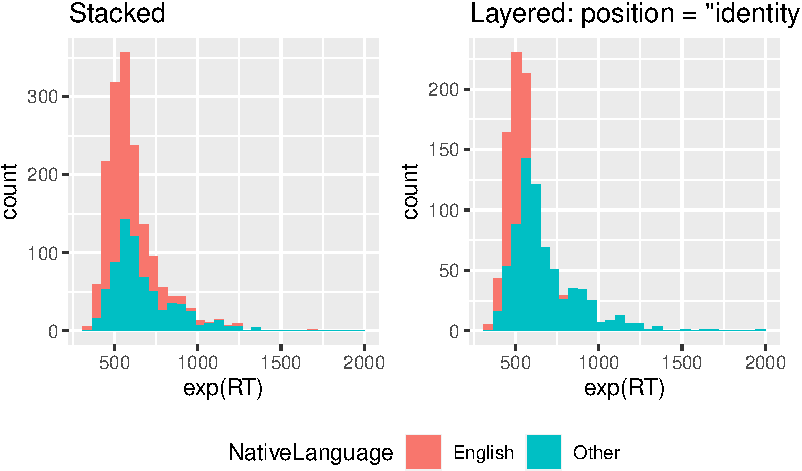
\includegraphics{_intro_r_slides_files/figure-pdf/unnamed-chunk-21-1.pdf}

}

\end{figure}

\hypertarget{global-and-local-aesthetics}{%
\subsection{Global and local
aesthetics}\label{global-and-local-aesthetics}}

\begin{itemize}
\tightlist
\item
  in our final plot, the colour of the histograms is slightly
  transparent

  \begin{itemize}
  \tightlist
  \item
    we can control this by adding the argument \texttt{alpha\ =\ 0.3} to
    \texttt{geom\_histogram()}
  \item
    alpha takes any other value between 0 and 1
  \end{itemize}
\end{itemize}

\begin{tcolorbox}[enhanced jigsaw, colbacktitle=quarto-callout-tip-color!10!white, rightrule=.15mm, toptitle=1mm, bottomtitle=1mm, breakable, leftrule=.75mm, toprule=.15mm, left=2mm, coltitle=black, opacitybacktitle=0.6, title=\textcolor{quarto-callout-tip-color}{\faLightbulb}\hspace{0.5em}{Aufgabe~\ref{exm-local}: Histogram transparency}, colback=white, titlerule=0mm, arc=.35mm, bottomrule=.15mm, opacityback=0, colframe=quarto-callout-tip-color-frame]

\begin{example}[]\protect\hypertarget{exm-local}{}\label{exm-local}

~

Play around with the transparency of the histogram geom. Choose the
alpha-value you prefer. The output should look something like this:

\begin{figure}[centre]

{\centering 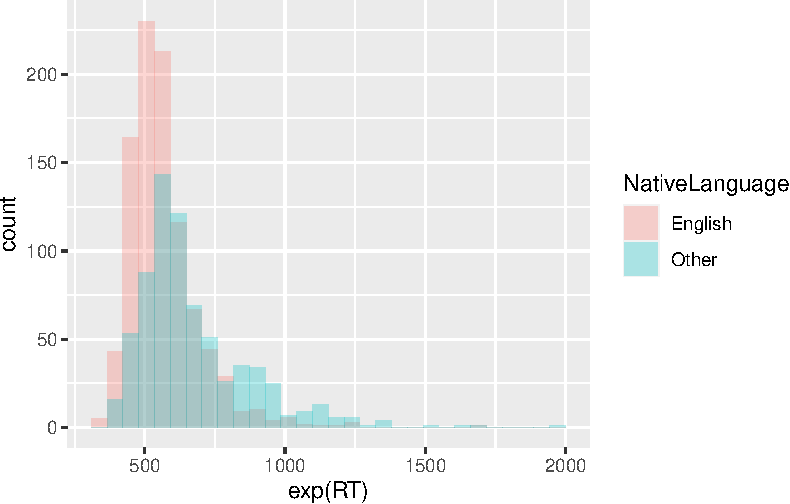
\includegraphics{_intro_r_slides_files/figure-pdf/unnamed-chunk-22-1.pdf}

}

\end{figure}

\end{example}

\end{tcolorbox}

\hypertarget{customising-our-plot}{%
\subsection{Customising our plot}\label{customising-our-plot}}

\begin{itemize}
\item
  we can improve our axis and legend labels, and also add titles using
  the \texttt{labs()} function
\item
  let's also use the function \texttt{scale\_fill\_colorblind()} from
  the \texttt{ggthemes} package

  \begin{itemize}
  \tightlist
  \item
    this creates colourblind-safe colours
  \end{itemize}
\item
  we'll also use the \texttt{theme\_minimal()} function from
  \texttt{ggplot2}; what does this do?
\item
  try to add the following to your plot

  \begin{itemize}
  \tightlist
  \item
    change the labels accordingly
  \item
    and add meaningful comments to the code using \texttt{\#}
  \end{itemize}
\end{itemize}

\begin{Shaded}
\begin{Highlighting}[]
\FunctionTok{labs}\NormalTok{(}\AttributeTok{title =} \StringTok{"Plot title"}\NormalTok{,}
     \AttributeTok{x =} \StringTok{"x{-}axis label"}\NormalTok{,}
     \AttributeTok{y =} \StringTok{"y{-}axis label"}\NormalTok{) }\SpecialCharTok{+}
  \FunctionTok{scale\_fill\_colourblind}\NormalTok{() }\SpecialCharTok{+}
  \FunctionTok{theme\_minimal}\NormalTok{()}
\end{Highlighting}
\end{Shaded}

\hypertarget{commenting}{%
\subsection{Commenting}\label{commenting}}

\begin{itemize}
\tightlist
\item
  the code and plot should look something like this:
\end{itemize}

\begin{Shaded}
\begin{Highlighting}[]
\CommentTok{\# histogram of reaction times by native language}
\FunctionTok{ggplot}\NormalTok{(}\AttributeTok{data =}\NormalTok{ df\_lexdec) }\SpecialCharTok{+}
  \FunctionTok{aes}\NormalTok{(}\AttributeTok{x =} \FunctionTok{exp}\NormalTok{(RT), }\AttributeTok{fill =}\NormalTok{ NativeLanguage) }\SpecialCharTok{+} \CommentTok{\# set aesthetics}
  \FunctionTok{labs}\NormalTok{(}\AttributeTok{title =} \StringTok{"Reaction times by L1"}\NormalTok{,}
     \AttributeTok{x =} \StringTok{"Reaction times (ms)"}\NormalTok{) }\SpecialCharTok{+}
  \FunctionTok{geom\_histogram}\NormalTok{(}\AttributeTok{position =} \StringTok{"identity"}\NormalTok{, }\AttributeTok{alpha =} \FloatTok{0.3}\NormalTok{) }\SpecialCharTok{+}
  \FunctionTok{scale\_fill\_colorblind}\NormalTok{() }\SpecialCharTok{+} \CommentTok{\# make fill colorblind friendly}
  \FunctionTok{theme\_minimal}\NormalTok{() }\CommentTok{\# set plot theme}
\end{Highlighting}
\end{Shaded}

\begin{figure}[centre]

{\centering 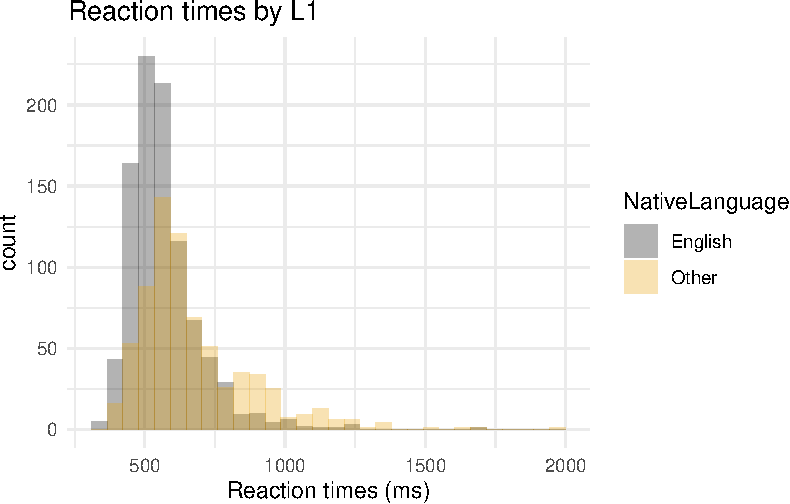
\includegraphics{_intro_r_slides_files/figure-pdf/unnamed-chunk-24-1.pdf}

}

\end{figure}

\hypertarget{saving-plots}{%
\subsection{Saving plots}\label{saving-plots}}

\begin{itemize}
\tightlist
\item
  we can store plots in our Environment, just like we can store numbers
  and data as objects

  \begin{itemize}
  \tightlist
  \item
    you can name objects anything you want
  \item
    but it's wise to make the name meaningful (e.g., \emph{not}
    \texttt{fig1} or \texttt{xyz})
  \end{itemize}
\item
  let's name this plot \texttt{fig\_lexdec\_rt}, for ``figure lexical
  decision task reaction times''
\end{itemize}

\begin{tcolorbox}[enhanced jigsaw, colbacktitle=quarto-callout-tip-color!10!white, rightrule=.15mm, toptitle=1mm, bottomtitle=1mm, breakable, leftrule=.75mm, toprule=.15mm, left=2mm, coltitle=black, opacitybacktitle=0.6, title=\textcolor{quarto-callout-tip-color}{\faLightbulb}\hspace{0.5em}{Aufgabe~\ref{exm-save}: \texttt{ggplot2} review}, colback=white, titlerule=0mm, arc=.35mm, bottomrule=.15mm, opacityback=0, colframe=quarto-callout-tip-color-frame]

\begin{example}[]\protect\hypertarget{exm-save}{}\label{exm-save}

~

\begin{enumerate}
\def\labelenumi{\arabic{enumi}.}
\tightlist
\item
  Save our final plot as an object called \texttt{fig\_lexdec\_rt}
\end{enumerate}

\end{example}

\end{tcolorbox}

\hypertarget{barplots}{%
\subsection{Barplots}\label{barplots}}

\begin{itemize}
\tightlist
\item
  copy the code for your histogram
\item
  make the following changes to render our barplot

  \begin{itemize}
  \tightlist
  \item
    remove the name assignment (\texttt{fig\_lexdec\_rt})
  \item
    on the x-axis we want \texttt{NativeLanguage}
  \item
    replace \texttt{geom\_histogram()} with \texttt{geom\_bar()}

    \begin{itemize}
    \tightlist
    \item
      remove the arguments for the histogram (not position or alpha)
    \end{itemize}
  \item
    change the labels accordingly
  \item
    save the plot as an object with some meaningful name (e.g.,
    \texttt{fig\_lexdec\_l1})
  \end{itemize}
\end{itemize}

\hypertarget{section-1}{%
\subsection{}\label{section-1}}

\begin{itemize}
\tightlist
\item
  the plot should look something like this:
\end{itemize}

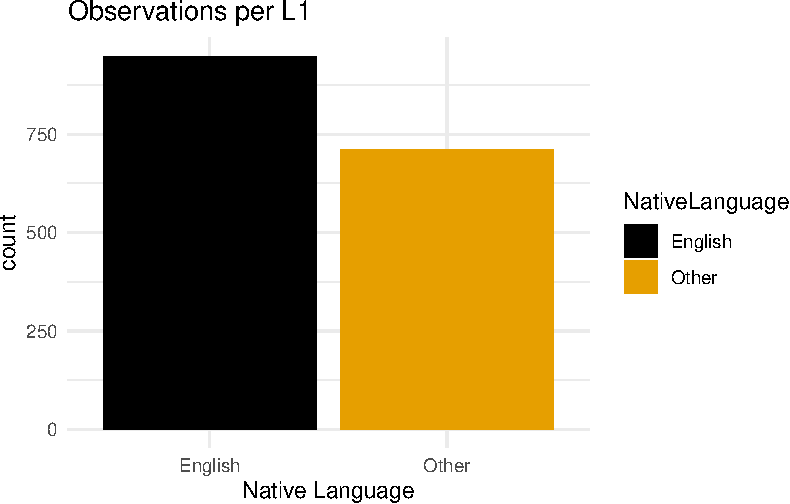
\includegraphics{_intro_r_slides_files/figure-pdf/unnamed-chunk-26-1.pdf}

\hypertarget{combining-plots}{%
\subsection{Combining plots}\label{combining-plots}}

\begin{itemize}
\tightlist
\item
  one reason to save your plot as an object is so that we can call on it
  later

  \begin{itemize}
  \tightlist
  \item
    i.e., you can produce the plot at one point in your document, but
    decide to only print it in the rendered report lower down
  \end{itemize}
\item
  another reason is so that we can combine multiple plots

  \begin{itemize}
  \tightlist
  \item
    this can be done with a variety of packages
  \item
    but let's try it with the \texttt{patchwork} package
  \item
    use \texttt{+} to connect two plots side-by-side
  \item
    or \texttt{/} to present them one on top of the other
  \end{itemize}
\end{itemize}

\hypertarget{combining-plots-with}{%
\subsubsection{\texorpdfstring{Combining plots with
\texttt{+}}{Combining plots with +}}\label{combining-plots-with}}

\begin{Shaded}
\begin{Highlighting}[]
\NormalTok{fig\_lexdec\_rt }\SpecialCharTok{+}\NormalTok{ fig\_lexdec\_l1}
\end{Highlighting}
\end{Shaded}

\begin{figure}[H]

{\centering 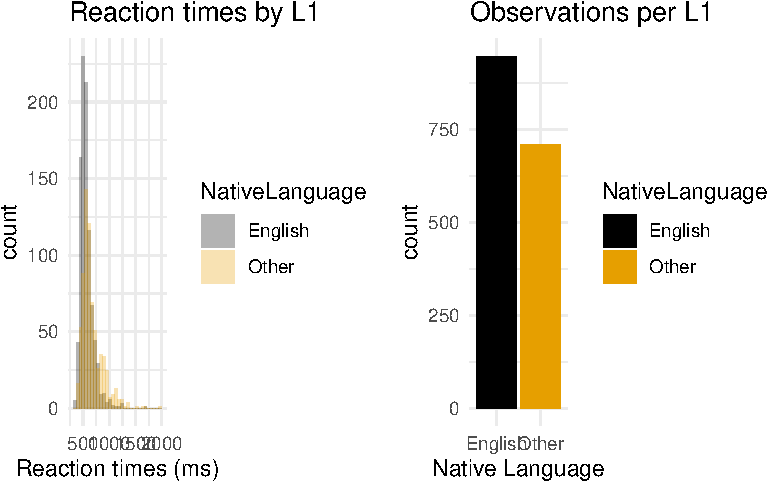
\includegraphics{_intro_r_slides_files/figure-pdf/unnamed-chunk-27-1.pdf}

}

\end{figure}

\hypertarget{combining-plots-with-1}{%
\subsubsection{\texorpdfstring{Combining plots with
\texttt{/}}{Combining plots with /}}\label{combining-plots-with-1}}

\begin{Shaded}
\begin{Highlighting}[]
\NormalTok{fig\_lexdec\_rt }\SpecialCharTok{/}\NormalTok{ fig\_lexdec\_l1}
\end{Highlighting}
\end{Shaded}

\begin{figure}[H]

{\centering 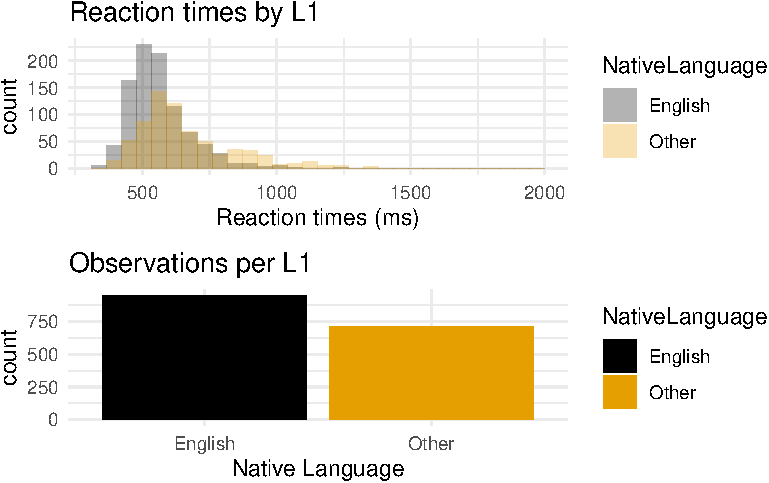
\includegraphics{_intro_r_slides_files/figure-pdf/unnamed-chunk-28-1.pdf}

}

\end{figure}

\hypertarget{deciding-on-a-geom}{%
\section{Deciding on a geom}\label{deciding-on-a-geom}}

\begin{itemize}
\tightlist
\item
  why do we use histogram for reaction times, and a barplot for native
  language?
\item
  what types of variables are these?

  \begin{itemize}
  \tightlist
  \item
    reaction time is continuous
  \item
    native language is categorical
  \end{itemize}
\item
  we use histograms to visualise distributions of \emph{continuous}
  variables
\item
  we use barplots to visualise distributions of \emph{cateogrical}
  variables
\item
  knowing what we want to visualise (e.g., distributions) and what type
  of variable we have (i.e., continuous, categorical) helps us decide
  which type of plot to produce
\item
  often, trying to draw your plot on paper before you start in R is a
  good idea (I often do this, too)
\end{itemize}

\hypertarget{exercises}{%
\section{Exercises}\label{exercises}}

\begin{enumerate}
\def\labelenumi{\arabic{enumi}.}
\item
  Reproduce our histogram as a \emph{density plot} by replacing
  \texttt{geom\_histogram()} with \texttt{geom\_density()}

  \begin{itemize}
  \tightlist
  \item
    what does this type of plot show?
  \end{itemize}
\item
  Produce a barplot that shows the number of observations per word class
  (hint: you'll need the variable \texttt{Class} from our dataset).
\item
  Print your density plot and class barplot one on top of the other
  using the \texttt{patchwork} package
\end{enumerate}

\hypertarget{section-2}{%
\subsection{}\label{section-2}}

\begin{enumerate}
\def\labelenumi{\arabic{enumi}.}
\setcounter{enumi}{3}
\tightlist
\item
  Reproduce the following plots as exactly as you can (hint: you will
  need the \texttt{position\ =\ "dodge"} argument):
\end{enumerate}

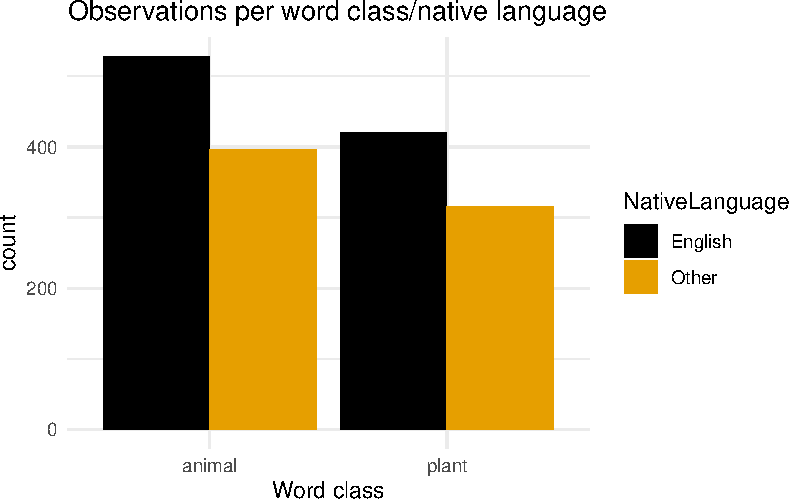
\includegraphics{_intro_r_slides_files/figure-pdf/unnamed-chunk-29-1.pdf}

\hypertarget{heutige-ziele-1}{%
\section*{Heutige Ziele}\label{heutige-ziele-1}}

Today we learned\ldots{}

\begin{itemize}
\tightlist
\item
  what data frames are
\item
  the difference between categorical and continuous data
\item
  how to produce plots with \texttt{ggplot}
\item
  choose the right plot for our data
\end{itemize}

\hypertarget{session-info}{%
\section*{Session Info}\label{session-info}}
\addcontentsline{toc}{section}{Session Info}

Hergestellt mit R version 4.3.0 (2023-04-21) (Already Tomorrow) und
RStudioversion 2023.3.0.386 (Cherry Blossom).

\begin{Shaded}
\begin{Highlighting}[]
\FunctionTok{sessionInfo}\NormalTok{()}
\end{Highlighting}
\end{Shaded}

\begin{verbatim}
R version 4.3.0 (2023-04-21)
Platform: aarch64-apple-darwin20 (64-bit)
Running under: macOS Ventura 13.2.1

Matrix products: default
BLAS:   /Library/Frameworks/R.framework/Versions/4.3-arm64/Resources/lib/libRblas.0.dylib 
LAPACK: /Library/Frameworks/R.framework/Versions/4.3-arm64/Resources/lib/libRlapack.dylib;  LAPACK version 3.11.0

locale:
[1] en_US.UTF-8/en_US.UTF-8/en_US.UTF-8/C/en_US.UTF-8/en_US.UTF-8

time zone: Europe/Berlin
tzcode source: internal

attached base packages:
[1] stats     graphics  grDevices utils     datasets  methods   base     

other attached packages:
 [1] magick_2.7.4     kableExtra_1.3.4 knitr_1.44       patchwork_1.1.3 
 [5] ggthemes_4.2.4   languageR_1.5.0  lubridate_1.9.2  forcats_1.0.0   
 [9] stringr_1.5.0    dplyr_1.1.3      purrr_1.0.2      readr_2.1.4     
[13] tidyr_1.3.0      tibble_3.2.1     ggplot2_3.4.3    tidyverse_2.0.0 

loaded via a namespace (and not attached):
 [1] utf8_1.2.3        generics_0.1.3    xml2_1.3.4        stringi_1.7.12   
 [5] hms_1.1.3         digest_0.6.33     magrittr_2.0.3    evaluate_0.21    
 [9] grid_4.3.0        timechange_0.2.0  fastmap_1.1.1     rprojroot_2.0.3  
[13] jsonlite_1.8.7    httr_1.4.6        rvest_1.0.3       fansi_1.0.4      
[17] viridisLite_0.4.2 scales_1.2.1      cli_3.6.1         rlang_1.1.1      
[21] munsell_0.5.0     withr_2.5.0       yaml_2.3.7        tools_4.3.0      
[25] tzdb_0.4.0        colorspace_2.1-0  webshot_0.5.4     here_1.0.1       
[29] pacman_0.5.1      vctrs_0.6.3       R6_2.5.1          lifecycle_1.0.3  
[33] pkgconfig_2.0.3   pillar_1.9.0      gtable_0.3.4      Rcpp_1.0.11      
[37] glue_1.6.2        systemfonts_1.0.4 xfun_0.39         tidyselect_1.2.0 
[41] rstudioapi_0.14   farver_2.1.1      htmltools_0.5.5   labeling_0.4.3   
[45] rmarkdown_2.22    svglite_2.1.1     compiler_4.3.0   
\end{verbatim}

\hypertarget{literaturverzeichnis}{%
\section*{Literaturverzeichnis}\label{literaturverzeichnis}}

\hypertarget{refs}{}
\begin{CSLReferences}{1}{0}
\leavevmode\vadjust pre{\hypertarget{ref-nordmann_applied_2022}{}}%
Nordmann, E., \& DeBruine, L. (2022). \emph{Applied Data Skills}.
Zenodo. \url{https://doi.org/10.5281/zenodo.6365078}

\leavevmode\vadjust pre{\hypertarget{ref-wickham_r_2023}{}}%
Wickham, H., Çetinkaya-Rundel, M., \& Grolemund, G. (2023). \emph{R for
{Data Science}} (2. Aufl.).

\end{CSLReferences}



\end{document}
